\section{Results}\label{sec:results}

\subsection{Connected peers}\label{subsec:connected-peers}
\begin{figure*}[!ht]
    \centering
    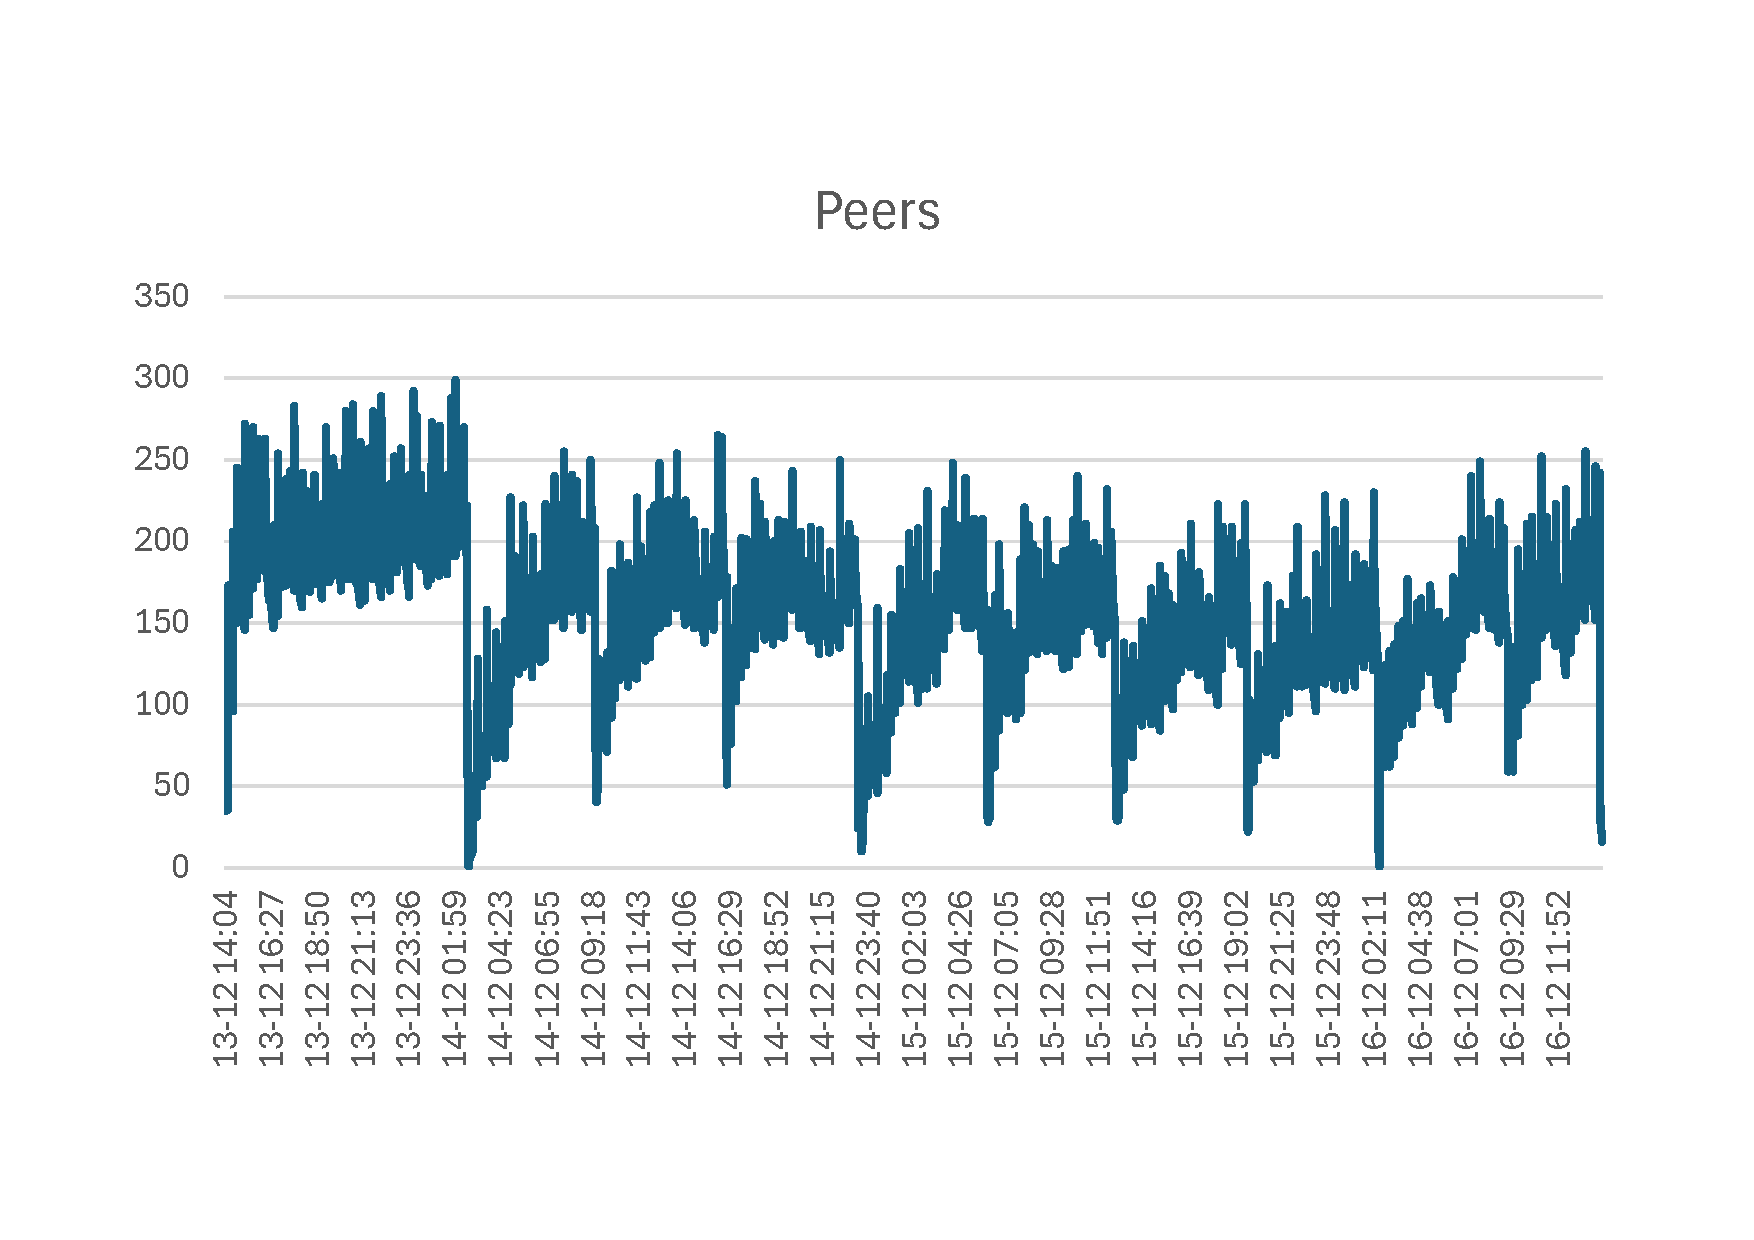
\includegraphics[scale = 0.5]{figures/conPeer2}
    \caption{The number of peers our node was connected to over the time of the experiment.
    Data points are collected every minute and the average amount of peers connected is 148.}
    \label{fig:peersconnected}
\end{figure*}
Throughout the experiment, we kept track of the number of peers our node was connected to.
The number of connected peers is shown in~\autoref{fig:peersconnected}.
Our node was connected to at most 299 peers at once, and the average was 148 peers.
The number of connected peers fluctuated widely throughout the experiment but continually rose for the first 12 hours.
Then, it would heavily drop and rise again.
This pattern would repeat, but after the first drop, it drops consistently every 7 hours.

\subsection{De-anonymization}\label{subsec:de-anonymization}
During the attack, we discovered a total of 1,195 unique peers.
The results of the de-anonymization attack are shown in~\autoref{tab:distribution}.
The table showcases the distribution of peers into four categories based on the heuristic described in~\autoref{subsec:inspirational-papers}.
Here, we see that 38.661\% of the peers we have encountered have had at least one validator that has been de-anonymized, meaning that the conditions from~\autoref{subsec:inspirational-papers} are fulfilled.
We also see that 5.941\% of the peers we discovered are subscribed to all 64 subnets.
We did not find validators on 35.314\% of the peers we discovered, meaning that we did not receive a single non-backbone attestation from any validator on these peers.
Lastly, we discovered that 20.084\% of peers did not fit into the other categories.
Failing to categorize a peer could be because the peer could be hosting a validator, but we could not, with enough confidence, say that to be the case based on our heuristic.


\begin{table}[]
    \centering
    \caption{Distribution of nodes into the four different categories.}
    \begin{tabular}{lll}
        \hline
        & \textbf{Nodes} & \textbf{Distribution} \\ \hline
        \textbf{Deanonymized validators} & 462            & 38.661\%                 \\
        \textbf{64 subnets}              & 71             & 5.941\%                  \\
        \textbf{No validators}           & 422              & 35.314\%               \\
        \textbf{Rest}                    & 240            & 20.084\%                 \\ \hline
        \\
    \end{tabular}
    \label{tab:distribution}
\end{table}


After the attack, we managed to de-anonymize a total of 492,959 validators corresponding to 28\% of the total number of validators in the Holesky network\footnote{As of 2024-01-08 seen on \href{https://holesky.beaconcha.in/}{holesky.beaconcha.in}}.
158,134 of these validators were non-unique, meaning that they had more than one IP address mapped to them over the duration of the attack.
The results are shown in~\autoref{tab:unique vals}.

In total, we logged 1,183 unique IP addresses.


\begin{table}[]
    \centering
    \caption{The number of validators located by our modified Prysm node. The first column indicates the total number of validators. The second column indicates validators with more than one IP address mapped to them.}
    \begin{tabular}{lll}
        \hline
        & \textbf{Validators} & \textbf{Non-Unique Validators} \\ \hline
        \textbf{Overall} & 492,959             & 158,134                        \\ \hline
        \\
    \end{tabular}
    \label{tab:unique vals}
\end{table}

\subsection{Validator Distribution}\label{subsec:validator-distribution}
\begin{figure*}[!ht]
    \centering
    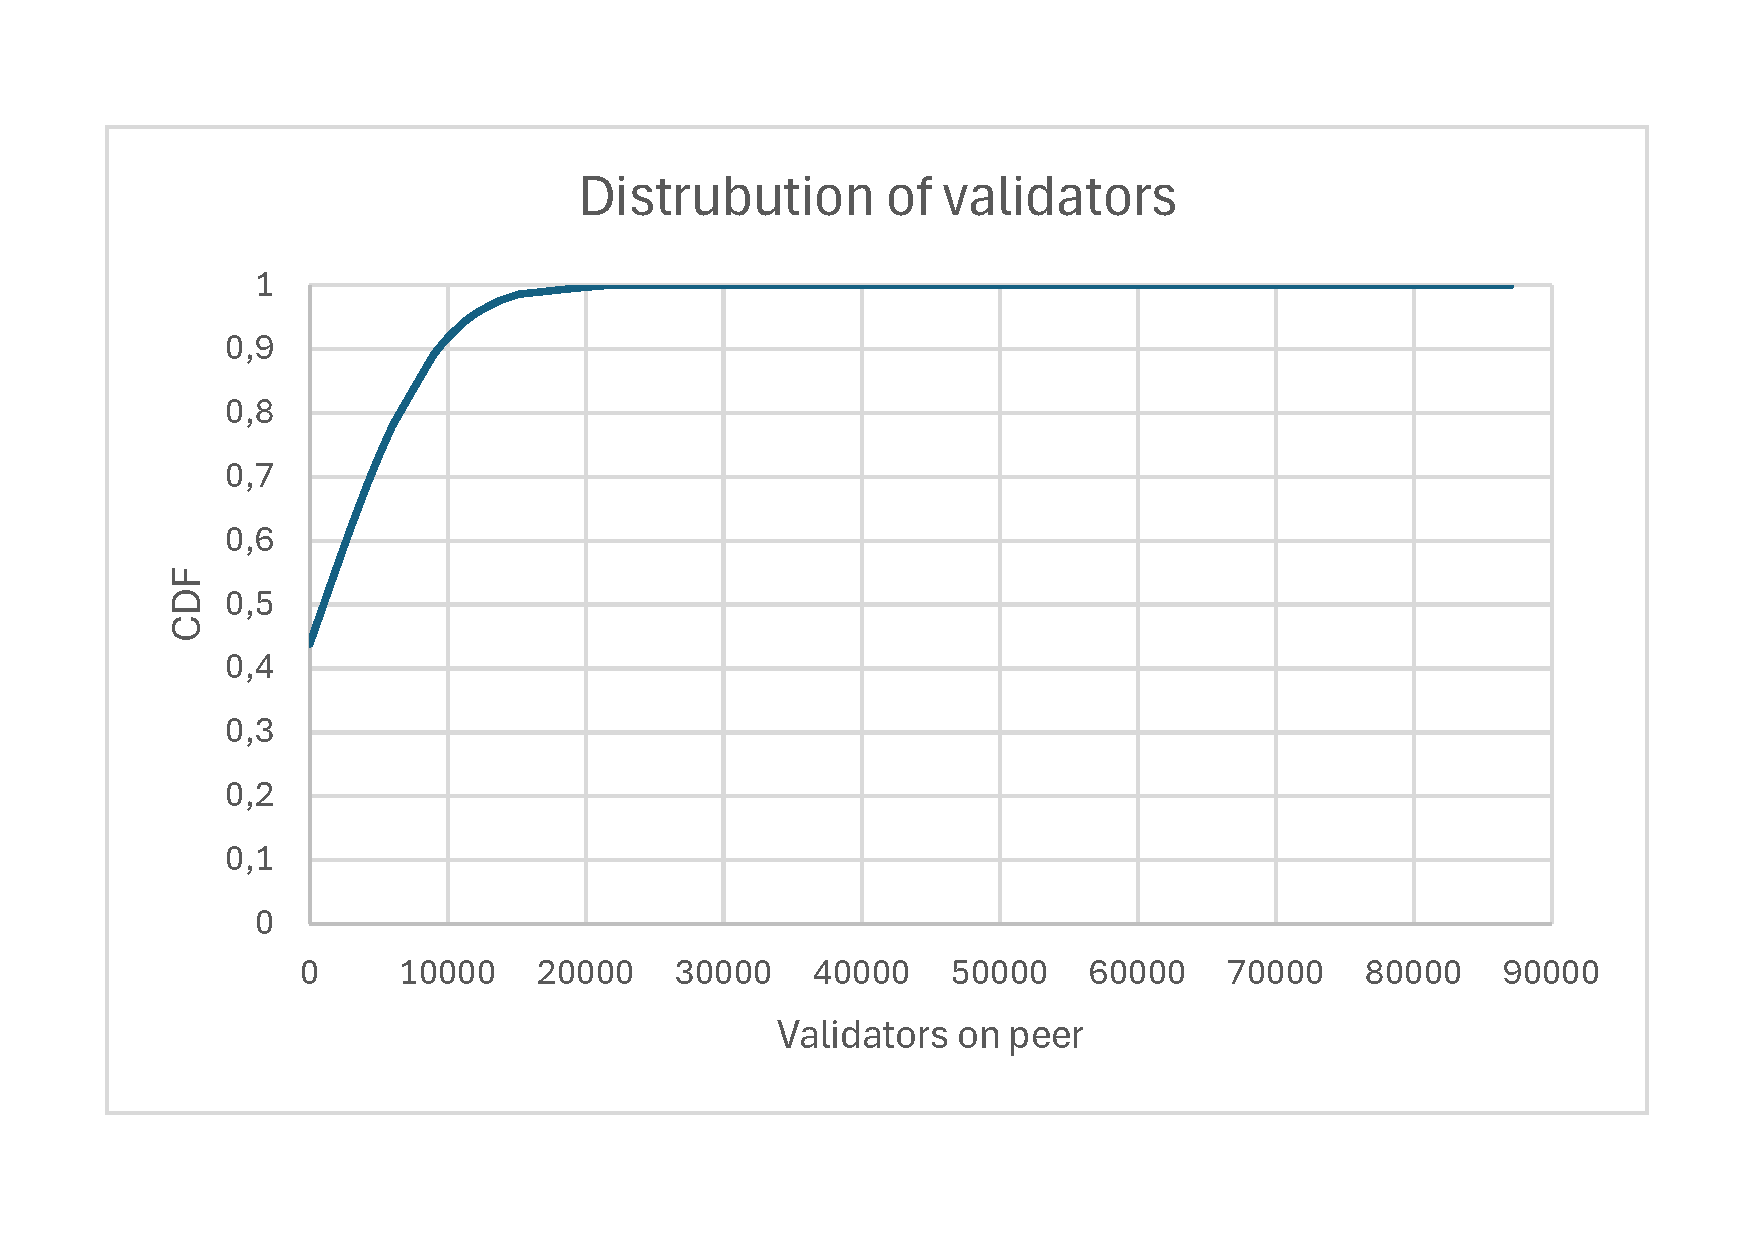
\includegraphics[scale = 0.45]{figures/distval}
    \caption{The cdf showing the distribution of validators on each peer}
    \label{fig:validatorsonpeers}
\end{figure*}
From all the peers we were connected to, we tallied the number of validators on each peer.
The cumulative distribution of validators on each peer is shown in~\autoref{fig:validatorsonpeers}.
Here, we can see that 57\% of the peers we connected to have at least one validator.
The amount of validators on each peer ranges from 0 to 87,028, with the average being 1,003 validators per peer.
We see that the most common number of validators on a peer is 1, with about 7\% of the found peers having only one validator.
We also saw that 110 and 400 were the most common numbers of validators on a peer once we got above 20 validators on a peer.
We found a total of 24 peers that had 10,000 or more validators on them.